\section{Homepage - assi informativi}
L’homepage rappresenta la vetrina del sito, è la sezione in cui l'utente 
tipicamente decide se visitare il sito o meno. 
Al fine di convincere l'utente è necessario fornire le informazioni 
necessarie a soddisfare le \quotes{6W}, ovvero una serie di domande
che tipicamente l'utente si pone quando approda alla homepage di un 
qualsiasi sito web.
    \begin{figure}[ht]
    \centering
    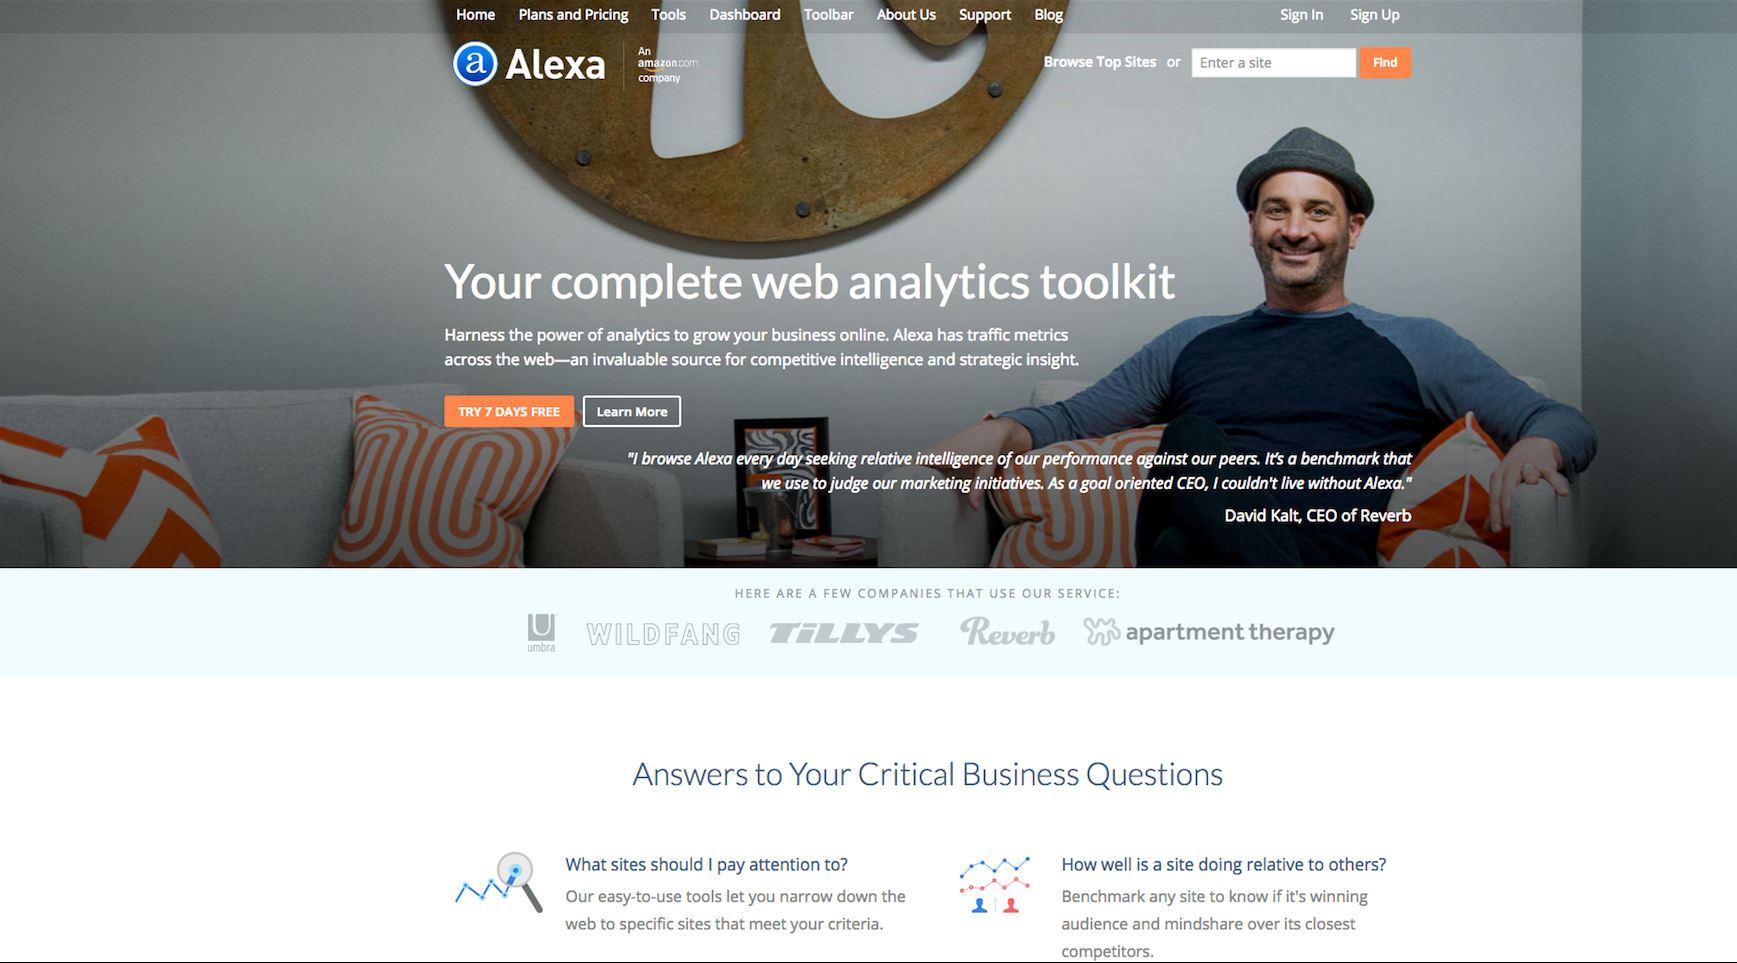
\includegraphics[scale=0.25,keepaspectratio]{{figure/3/home}.png}
    \caption{Homepage}
    \end{figure}
    \FloatBarrier 
  \subsection{Where}
\begin{center}

\textit{A che tipo di sito sono arrivato?}

Nella homepage del sito compare, in font sans serif di dimensione
più grande risepetto al resto del testo presente nella pagina, il motto: \\
\quotes{Your complete web analytics toolkit} \\
Grazie a questa informazione l'utente sa di trovarsi in un sito che offre
strumenti di ricerca per il web.

\end{center}
  \subsection{Who}\label{who}
\begin{center}

\textit{Chi rappresenta il sito?}


\end{center}
\begin{flushleft}
Il logo dell'azienda, il nome, e l'indicazione di appartenenza ad Amazon 
dicono chi rappresenta il sito. Importante notare come queste 
informazioni siano poste in una zona \quotes{calda} della pagina: risultano 
nell'angolo in alto a sinistra della forma ad \quotes{F} evidenziata 
dalle analisi di eyetracking. Per avere informazioni più specifiche sull'asse \textit{Who}
è necessario selezionare la sezione About nel menù di navigazione. \\
In generale l'asse \textit{Who} risulta soddisfatto. \\
Risultato : \textbf{8}
\end{flushleft}
  \subsection{Why}\label{why}
\begin{center}

\textit{Quali benefici offre il sito e quali sono le motivazioni per visitarlo?}

\end{center}
\begin{flushleft}
Come blurb al motto presente in Homepage viene spiegato quali benefici il sito 
possa offrire: \\
\quotes{an invaluable source for competitive intelligence and strategic insight}
\\
Per rendere più \quotes{umano} l'asse \quotes{Why}, e quindi convincere l'utente,
viene messo come sfondo della Homepage un CEO sorridente che utilizza i servizi di Alexa
per la sua azienda. A rimarcare ciò contribuisce la citazione sottostante al 
blurb appena descritto. Infine (sempre nella prima pagina)
vengono citate alcune aziende clienti di Alexa. Un'osservazione riguarda il contenuto
che, in questo caso, viene presentato in stile \quotes{slogan} e con poche informazioni
teniche e specifiche. Quest'ultima non è una buona prassi soprattutto perchè il target di utenza
per questa tipologia di siti è definito in partenza (vedi \ref{scopo}) e quindi
molto probabilmente gli utenti si aspettano delle informazioni più specifiche 
e potrebbero rimanere infastiditi dall'uso eccessivo di slogan. \\
Risultato : \textit{8.5}

\end{flushleft}
  \subsection{What}
\begin{center}

\textit{Cosa offre il sito?}

\end{center}
\begin{flushleft}
Questo asse non è subito visualizzabile in modo chiaro. Solo effetuando un 
primo scroll è possibile capire che strumenti di analisi web offre il sito.
Si sarebbe potuto evitare ciò riorganizzando meglio lo spazio della prima pagina senza scroll
o comunque sfruttando le colonne laterali che non vengono mai utilizzate nella homepage.
Le informazioni riguardanti l'asse \textit{What} non sono sempre organizzate in modo standard in 
tutte le pagine di scroll presenti in homepage:
\begin{itemize}
	\item la prima pagina di scroll utile le organizza a griglia;
	\item la seconda a lista;
	\item dalla terza pagina verticalmente (implica ulteriore scroll);
	\item dalla quinta ancora a lista fino all'ultima.
\end{itemize}
Queste diverse disposizioni
potrebbero affaticare l'utente nella navigazione della homepage. \\
Screenshot disponibile al path : \textit{figure/3/what0.png} \\
Un'altra osservazione
riguarda le immagini, in questo caso viene violata una convenzione web importante: 
\begin{center}
	\quotes{le immagini devono essere cliccabili}
\end{center}
Non tutte le immagini riguardanti l'asse \textit{What} sono cliccabili, l'unico modo 
di accedere alle funzionalità presentate è utilizzare il pulsante correlato 
che almeno risulta ben visibile e correttamente implementato (la zona cliccabile corrisponde a 
tutta la zona visibile). Le informazioni, anche se presentate in modo non ottimale,
risultano tuttavia esaustive.
    \begin{figure}[ht]
    \centering
    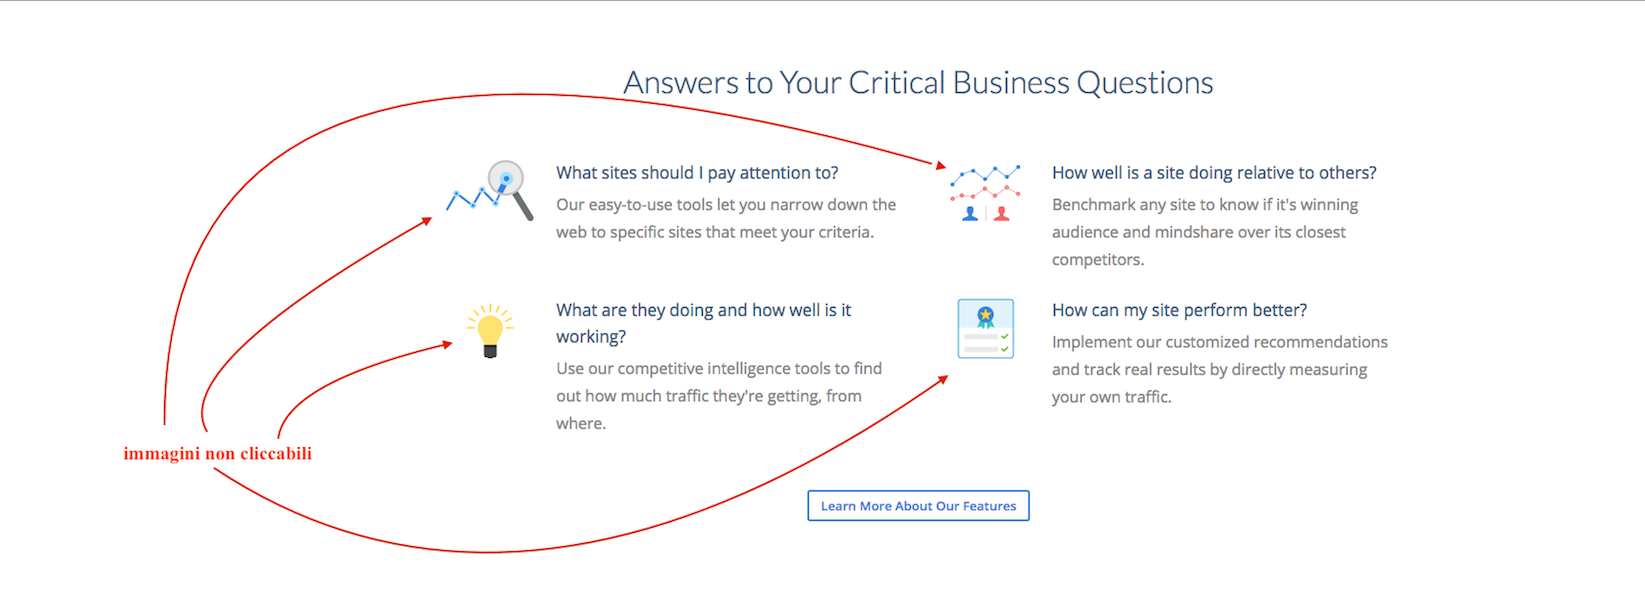
\includegraphics[scale=0.25,keepaspectratio]{{figure/3/what1}.png}
    \caption{Immagini non cliccabili}
    \end{figure}
    \FloatBarrier 
Risultato : \textbf{6}
\end{flushleft}
  \subsection{When}
\begin{center}

\textit{Quali sono le ultime novità? Quando è stato aggiornato l'ultima volta?}

\end{center}
  \subsection{How}\label{how}
\begin{center}

\textit{Come faccio ad arrivare alle sezioni principali?}

\end{center}
\begin{flushleft}
Il menù di navigazione non permette di muoversi agevolmente
in tutte le parti del sito in quanto molte sottosezioni sono \quotes{nascoste}
nell'utilizzo dei pulsanti (come spiegato in §\ref{sezioni}) compromettendo quasi totalmente la navigazione. \\
Risulta oneroso
consultare e cercare le informazioni di cui l'utente necessita.\\
Una possibile soluzione consiste in:
\begin{itemize}
	\item ridurre le molte pagine di scroll, presenti nella maggior parte
delle sezioni, e creare delle sezioni 
a profondità maggiore rendendo l'attuale menù a tendina (con due livelli
 di profondità sarebbe sufficiente);
\item dare al menù una posizione
fissa rispetto al browser in modo che, anche nel caso si utilizzasse lo scrolling
verticale, sia sempre possibile per l'utente avere le informazioni relative all'asse
\textit{How}.
\end{itemize}
    \begin{figure}[ht]
    \centering
    
\includegraphics[scale=0.38,keepaspectratio]{{figure/3/how0}.png}
    \caption{Homepage - Menù ad un solo livello}
    \end{figure}
    \FloatBarrier 
Risultato : \textit{3}
\end{flushleft}
